\documentclass[conference]{IEEEtran}
\IEEEoverridecommandlockouts
% The preceding line is only needed to identify funding in the first footnote. If that is unneeded, please comment it out.
\usepackage{
    algorithmic,
    amsmath,
    amssymb,
    amsfonts,
    enumitem,
    graphicx,
    hyperref,
    textcomp,
    xcolor,
}
\usepackage[
    style=ieee
]{biblatex}

\addbibresource{references.bib}

\def\papertitle{Smart Room Air Conditioner}
\def\authoronename{Josep Marcello}
\def\authoroneemail{13519164@std.stei.itb.ac.id}
\def\authortwoname{Jeremia Bachtera}
\def\authortwoemail{13519188@std.stei.itb.ac.id}
\def\authorthreename{Jeane Erwansyah}
\def\authorthreeemail{13519116@std.stei.itb.ac.id}
\def\citycountry{Bandung City, Indonesia}
\def\department{School of Electrical Engineering and Informatics}
\def\organization{Institut Teknologi Bandung}

\def\BibTeX{{\rm B\kern-.05em{\sc i\kern-.025em b}\kern-.08em
    T\kern-.1667em\lower.7ex\hbox{E}\kern-.125emX}}
\begin{document}

\title{\papertitle}

\author{
    \IEEEauthorblockN{
        \authoronename\IEEEauthorrefmark{1},
        \authortwoname\IEEEauthorrefmark{2}, and \authorthreename\IEEEauthorrefmark{3}}
    \IEEEauthorblockA{\department,
        \organization\\
        \citycountry\\
        Email: \IEEEauthorrefmark{1}\authoroneemail,
        \IEEEauthorrefmark{2}\authortwoemail,
        \IEEEauthorrefmark{3}\authorthreeemail
    }
}
\maketitle

\begin{abstract}
    Air quality is an important aspect of a room.
    It affects the health, comfort, and
    productivity of the occupants. This paper
    presents an Internet-of-Things based system
    that can be used to monitor the air quality of
    a room and the outside air, and control the
    door/window of the room in hope of achieving a
    better air quality. The system will be able to
    monitor the air quality of a room, with
    temperature and humidity as the indicators,
    using DHT22 sensor; and the outside, with
    carbon dioxide (CO2) ppm as the indicator,
    using MQ135 sensor; and ESP32 as the
    microprocessor. The system also utilizes
    Time Series KMeans (TSKM) to determine the
    quality of the indicators, to decide whether
    to open or close the door.
\end{abstract}

\begin{IEEEkeywords}
    Air quality, Internet-of-Things, ESP32, DHT22, MQ135, Time Series KMeans, Web Application
\end{IEEEkeywords}

\section{Introduction}
One's room air quality is an important factor in one's health and productivity.
According to \cite{productivity_air_quality_wargocki_2000}, the air quality affects productivity in offices. Furthermore, Wargocki et al. also concluded that the performance is estimated to increase on average by 1.5\% per 10\% decrease of dissatisfaction with the air quality and 1.9\% increase for every two-fold pollution load decrease. This shows the importance of regulating the air quality of a room.
Not only that, according to \cite{indoor_air_quality_stafford_2015}, we spend around 90\% of our time indoors, thus the room/building we are in has the ability to influence our health and productivity.
Combined with the current post-pandemic situation, where some of the works are done from home, the air quality of one's room is more important than ever.

In this paper, we present a system that monitors the air quality of a room and the outside, and uses those informations to make decision about when to open and close doors/windows.
For ease of use, in this paper, we will use the term "door" to refer to both doors and windows.
This system should work well, especially with majority of college students, especially Indonesia, live in boarding houses, which usually have small rooms with only one door and one window. This condition affects the circulation of the air quality, and thus may also impacts in their academic performance, as stated in \cite{indoor_air_quality_stafford_2015}.

In this paper, we will use humidity and temperature as indicators of indoor air quality while CO2 (\textit{carbon dioxide}) as indicators of outdoor air quality.
Humidity and temperature are chosen as the indicators of the indoor air quality due to their significance in impacting it's inhabitant's comfort in the room, while also considering the outdoor quality, as the outdoor air quality may not be any better than the indoor air.
To measure these indicators, we will use DHT22 sensor to measure both humidity and temperature, and MQ135 sensor to measure CO2. We will also use a servo motor to open and close the door.

To implement the system, we will utilize the Internet of Things (IoT) technology.
The microprocessor, ESP32, that monitors and control the room will be connected to the internet via WiFi, and will be connected to a web application.

The web application acts as the interface for the user to interact with the system.
The web application will be able to display the current air quality of the room and the outside, and the status of the door; send commands to open and close the door manually; and send notifications to the user's phone about the state of the system.

We will use KMeans algorithm to cluster the data from the sensors to determine whether the door should be opened or closed. This algorithm is chosen because it is simple and easy to implement, and it is also suitable for this use case, as we will explain in the next section.
\section{Literature Review}

This section presents a literature review and definitions of key concepts and
components that is used by the proposed system.

\subsection{Air Quality}

Air quality refers to how healthy and comfortable the air is. In this paper, the
quality level is determined by:
\begin{itemize}
	\item the parts per million (ppm) of CO$_2$,
	\item temperature, and
	\item humidity level (in percent)
\end{itemize}
of the air.

In 2020, the Water and Air Quality Bureau of Health Canada proposed a long-term
exposure limit for CO$_2$ should not exceed 1000 ppm (based on 24 hours
average). Exposure to high CO$_2$ ppm can lead to health issues, such as dry
eyes and tight chest, and also neurological effects that affect cognitive
perofrmance. Some studies have shown that decrease in CO$_2$ ppm leads to better
better task performance and decrease in sick building syndrome
symptoms\cite{co2_ppm_max}.

The comfortable temperature and humidity in this paper is determined by the
average temperature range and average humidity of Bandung City, West Java,
Indonesia. According to weather-and-climate.com, the temperature in Bandung
usually ranges from 22\textdegree C to 30\textdegree C\cite{temperature_max}.
For humidity, the same source is used but the city is in Bogor, West Java
because there's no humidity data in Bandung and Bogor has geographic similarity
to Bandung which includes the humidity. According to said source, Bogor has an
average humidity of 80\%\cite{humidity_max}.

%% JOSEP: MIGHT NOT FIT FOR CHAPTER 2
% Based on the proposed maximum CO$_2$ ppm by Water and Air Quality Bureau of
% Health Canada, to have a good air quality, the CO$_2$ ppm has to be as low as
% possible. It is also observed to have a good air quality, the humidity and
% temperature should be a ``perfect'' value which is not be too high.

\subsection{Internet of Things}

Internet of Things (``IoT'') are interconnections of physical objects that has
the ability to transfer data over a network, might it be wired or wireless
\cite{iot}. IoT usually consists of edge devices connected with sensors to collect
data and then transmit them over internet. Data collected by sensors are usually
transmitted over internet to be processed by stronger computers or servers.

\subsection{K-means Clustering}

K-means clustering is one of the algorithms that can be used for
unsupervised learning in machine learning. With unsupervised learning,
the engineer doesn't have to label each data sample, instead the machine will
learn from the data and apply label in its own. This is very helpful when
the given dataset is unlabeled and comes in high quantity.

K-means clustering is also known as squared-error clustering because the
objective is to obtain a partition which, for a fixed number of clusters,
minimizes the square-error \cite*{clustering_fariska}. Square-error is the sum
of the Euclidean distance between each data sample in a cluster and its cluster
center.

In k-means clustering, clusters will be created and using the means of each
samples in the cluster. Then, the machine learning algorithm will label a data
sample with a cluster where the mean of said cluster is the to the sample's
data.

The alogrithm of training an ML model using k-means clustering to create a model
with $k$ clusters is as follows\cite{clustering_fariska}:
\begin{enumerate}
	\item randomly choose $k$ data points from the dataset $D$,
	\item repeat until convergence (no change in cluster):
	      \begin{enumerate}
		      \item assign (or reassign if needed) each data point to a cluster
		            where it is the most similar (based on the value).
		      \item update the cluster means.
	      \end{enumerate}
\end{enumerate}

\subsection{ESP32}

ESP32 is a family of chips with low-cost and low-power SoC (system on a chip)
with Wi-Fi and Bluetooth by Espressif systems \cite{esp32_net}. ESP32 has a single
32-bit processor with up 2 cores and clock speed of up to 240 MHz. This results
in a performance of up to 600 DMIPS. Additionally, all ESP32 models have 448 KiB
of ROM and 520 KiB of SRAM\cite{esp32_datasheet}.

ESP32 systems can be connected wirelessly using Bluetooth or Wi-Fi. For Wi-Fi,
ESP32 fully supports TCP/IP and 802.11 b/g/n Wi-Fi MAC protocol. While on the
Bluetooth side, ESP32 supports Bluetooth V4.2 BR/EDR and Bluetooth LE (low energy).
ESP32 can also be connected using USB through serial port\cite{esp32_datasheet}.

Programming and flashing ESP32 can be done using ESP-IDF (Espressif IoT
Development Framework). ESP-IDF the official IoT development framework for ESP32
created by Espressif Systems. Although other frameworks and IDE, such as
platform.io and Arduino IDE, also supports creating and loading programs for and
to ESP32.

\subsection{Message Queuing Telemetry Transport Broker (MQTT)}

MQTT is an OASIS standard messaging protocol that's usually used for IoT
development. It is also known as ISO/IEC 20922:2016. MQTT is designed to be
light-weight, open, simple, and easy to implement\cite{mqtt_iso}. MQTT runs over
TCP/IP or other networking protocol which provides the same characteristics as
TCP/IP (e.g. TLS).

MQTT has the following features:
\begin{itemize}
	\item uses pub/sub messaging pattern which provides one-to-many message
	      distribution,
	\item a messaging transport that's agnotic to the content payload,
	\item has the three qualities of message delivery: at-most-once,
	      at-least-once, exactly-once, and
	\item uses broker and topics.
\end{itemize}
The features and characteristics of MQTT makes it suitable for IoT usage
where the embedded computer is usually low-powered and might have unreliable
network.

MQTT also has some additional security features, such as the use of TLS
for transport protocol. MQTT also supports modern authentication protocols, such
as OAuth\cite{mqtt_org}.

\subsection{Apache Kafka}

Apache Kafka is an open-source message queue system by Apache Software
Foundation. Its usage is similar to MQTT where it has a broker and topics and
the clients send messages in a pub/sub manner. The difference between Kafka and
MQTT lies in the implementation. MQTT is a standard, Kafka is already
the implementation. Kafka brokers store message logs which means client can
consume it later (i.e. not realtime) as long as the message log still exists.
Also, Kafka can have multiple brokers, whereas MQTT really depends on the
implementation.

\subsection{Redis}

Redis is a NoSql database that uses a key-value schema. Redis saves its data
in-memory\footnote{Redis has Redis Persistance to periodically save data to
	secondary memory as backup}, which means it's perfect to be used for
caching. Other than for caching, Redis can also used to save state between
application. Because it has a fast I/O (when ignoring network), multiple
instances of an application can connect to the same Redis instance and share
their state through Redis.

\subsection{InfluxDB and Telegraf}

InfluxDB is a NoSql database with high read and write performance. Data can be
written and read in realtime. It is also included ETL (extract, transform, and
load), monitoring, user dashboard, and data visualization tools out of the box.
The features of InfluxDB makes it a perfect DB for saving IoT sensor data which
is captured at a fast rate. In InfluxDB, tables are similar to measurements and
databases are similar to buckets.

InfluxDB also has features for security. It includes authentication where user
needs to login before they can access the dashboard. It also has authorization
to access its buckets in the form of API token.

To insert data to InfluxDB buckets, its user can use the InfluxDB API, SDK, or
Telegraf. Telegraf is a server agent to collect data from systems and sensors.
Telegraf can be attached to MQTT to retrieve data from MQTT and then save them
directly to InfluxDB.

\subsection{Apache Spark}

Apache Spark is a product of Apache Software Foundation. Apache Spark is mostly
used for big data processing. Spark is usually used for ETL processes for big
data. Apache Spark can also be used to train machine learning models in real
time.

Apache Spark is able to process large amount of data in relatively short time
because it uses primary memory to save temporary data instead of writing them to
a file. Apache Spark can also be distributed accross machines spread all over
the world or be run in a multiprocess configuration in a single machine.
\section{Implementation}

\subsection{System Architecture}
The architecture of the system we proposed can be seen in
figure \ref{system-architecture}.
We can separate the deployment into 4 groups.
\begin{enumerate}
    \item The first one, the ESP32, are the physical device
          that gathers the air quality data and controls the door.
    \item Second, the Application Server are the primary brain
          of the whole system from collecting the data
          retrieved from the ESP32, saving the data, to
          managing the state of the system.
    \item Third, the SparkMachine, are the processor of data
          that processes the data into more meaningful
          informations for the user, such as minimum, maximum,
          and average values.
    \item Lastly, the User Device are users' devices that
          accesses the web application to interact with the
          system.
\end{enumerate}

\begin{figure*}
    \centering
    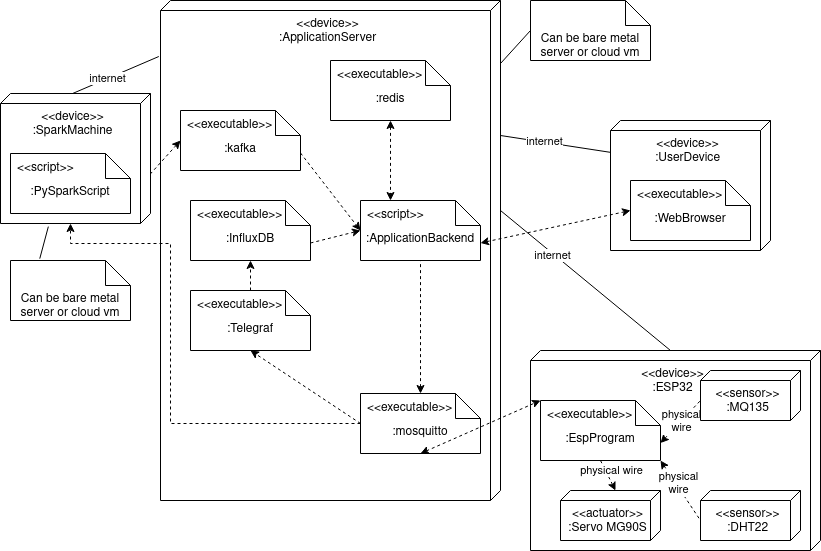
\includegraphics[scale=0.5]{resources/deployment-diagram.png}
    \caption{Deployment diagram of the smart room air conditioner}
    \label{system-architecture}
\end{figure*}

Flow-wise, the data gathered by the MQ135 and DHT22, in the
ESP32, are sent to the mosquitto, the MQTT broker, in the
Application Server.
There, the data are consumed by both Telegraf in the
Application Server to be saved into the InfluxDB, and
PySparkScript in the SparkMachine to be processed into
minimum, maximum, average, and median values.

The sensor data in InfluxDB and the processed data are then
used to be displayed as a statistic of the web application.
The sensor data are also used as training data for the KMeans
algorithm to determine the air quality level of each
indicators. The current average of each indicators are then
passed to the KMeans model to determine the current air
quality level of the room, thus determining whether the door
should be opened or closed.

\subsection{Experimental Setup}
In this section, we will describe the experimental setup of the proposed system.
There are two main spaces, which are a closed room and the outside of the room.
These two spaces are partitioned by a door and/or a window. Inside the room,
DHT22 sensor is placed to measure the temperature and humidity of the room.
Outside the room, MQ135 sensor is placed to measure the CO$_2$ ppm outside the room.
A servo motor is placed to open and close the door/window.
Experimental setup of the system can be seen in figure \ref{setup}.

\begin{figure}
    \centerline{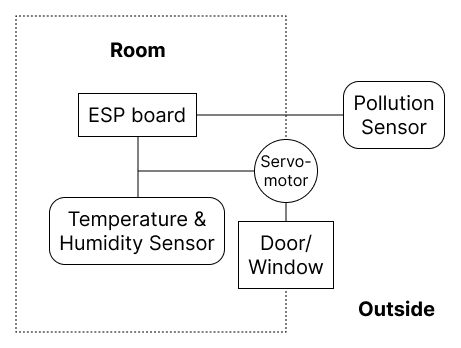
\includegraphics[scale=0.4]{resources/setup.png}}
    \caption{Experimental setup of the smart room air conditioner}
    \label{setup}
\end{figure}

Control setup of the system is when the door is open and all sensors are
indicating normal values or within an acceptable range. This system is will be
tested in the following scenarios:
\begin{enumerate}
    \item Using auto mode, a match will be lit and placed near the MQ135 sensor
          in order to increase the CO$_2$ ppm outside the room. The door should
          be closed to prevent bad air from coming in.
    \item Using auto mode, a match will be lit and placed near the DHT22 sensor
          to increase the temperature/humidity inside the room. The door should
          should be opened to let fresh air in.
    \item Using override mode, a match will be lit and placed near the MQ135
          sensor in order to increase the CO$_2$ ppm outside the room. If the door
          is opened, an email will be sent to warn the user to close the door.
    \item Using override mode, a match will be lit and placed near the DHT22
          sensor to increase the temperature/humidity inside the room. If the door
          is closed, an email will be sent to warn the user to open the door.
\end{enumerate}

\subsection{Machine Learning Model}
Since the data gathered by the sensors are time
series data, we will use Time Series KMeans (TSKM)
algorithm to cluster the data, that is provided in
python by
\href{https://tslearn.readthedocs.io/en/stable/}{\texttt{tslearn}} library.
KMeans algorithm are chosen because it is simple and
easy to implement, and it is also one of the most
popular clustering technique.

To train the model, we used the data gathered by the
sensors for 3 days, as the InfluxDB database stores,
from 2021-05-01 to 2021-05-03. Since the data,
especially from the MQ135 sensor were not too
accurate, we ``smoothened'' the data by using the
\href{https://pandas.pydata.org/docs/reference/api/pandas.DataFrame.rolling.html}{\texttt{rolling}} mean, which saves
the mean of the current rolling window of 120 data. The number
120 is chosen arbitarily to ensure the data is smooth enough,
but not too smooth that it loses its meaning. We also used 2
clusters for the model, as we only need to separate the data
into ``good'' and ``bad'' air quality.

The result of the training can be seen in
figure \ref{kmeans}. Due to use of clustering algorithm, we could not
determine the exact value of each indicators that is the
discriminant point that separates the ``good'' and ``bad''
air quality, but we can see that the ``good'' air quality is
represented by the lower part, and the ``bad'' air quality is
represented by the upper part.

We then implement the model into the system by passing each
indicator's current average value to the model to determine
the current air quality level of the room. The result of the
model is then used to determine whether the door should be
opened or closed using the following rules:
\begin{enumerate}
    \item If the CO$_2$ level is ``bad'', the door will not be
          opened, since we don't want any toxic particles to
          get in the room.
    \item If the CO$_2$ level is ``good'', we will check the
          next indicators, temperature and humidity. If
          either temperature or humidity is ``bad'', then the
          door will be opened, since we want to get fresh
          air into the room.
    \item If both temperature and humidity are ``good'',
          then the door will not be opened, since the air
          quality is already good.
\end{enumerate}

\begin{figure}
    \centerline{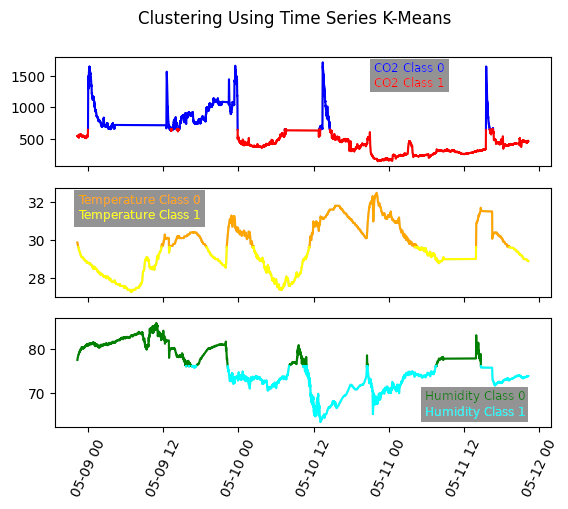
\includegraphics[scale=0.65]{resources/iot-clustering.png}}
    \caption{Time Series KMeans clustering result visualization}
    \label{kmeans}
\end{figure}

\section{Result and Discussion}
This section presents the results of the system,
and discusses the results.

\subsection{Result}
The results of the system can be seen in the web
application. The system can successfully gather the data from the
MQ135 and DHT22 sensors, and can display the data in
the web application, as seen in figure \ref{webapp-stats-view}.
There are a few time intervals to choose from to display the data.
The system can successfully open and close the door by
determining the current average of the indicators,
and act accordingly. As seen in figure \ref{webapp-home-view},
the web application is an user interface to control the system,
to change system mode, and to open or close the door remotely.
At the time of writing this paper, the alarm feature is not yet functional.
Figure \ref{webapp-alerts-view} shows the alerts view of the web application.
The alerts shown are alerts that sent within the last 12 hours.
A token must be inputted in the web application to be able to control the system,
to view statistics, and to view alerts.

\begin{figure}
      \centerline{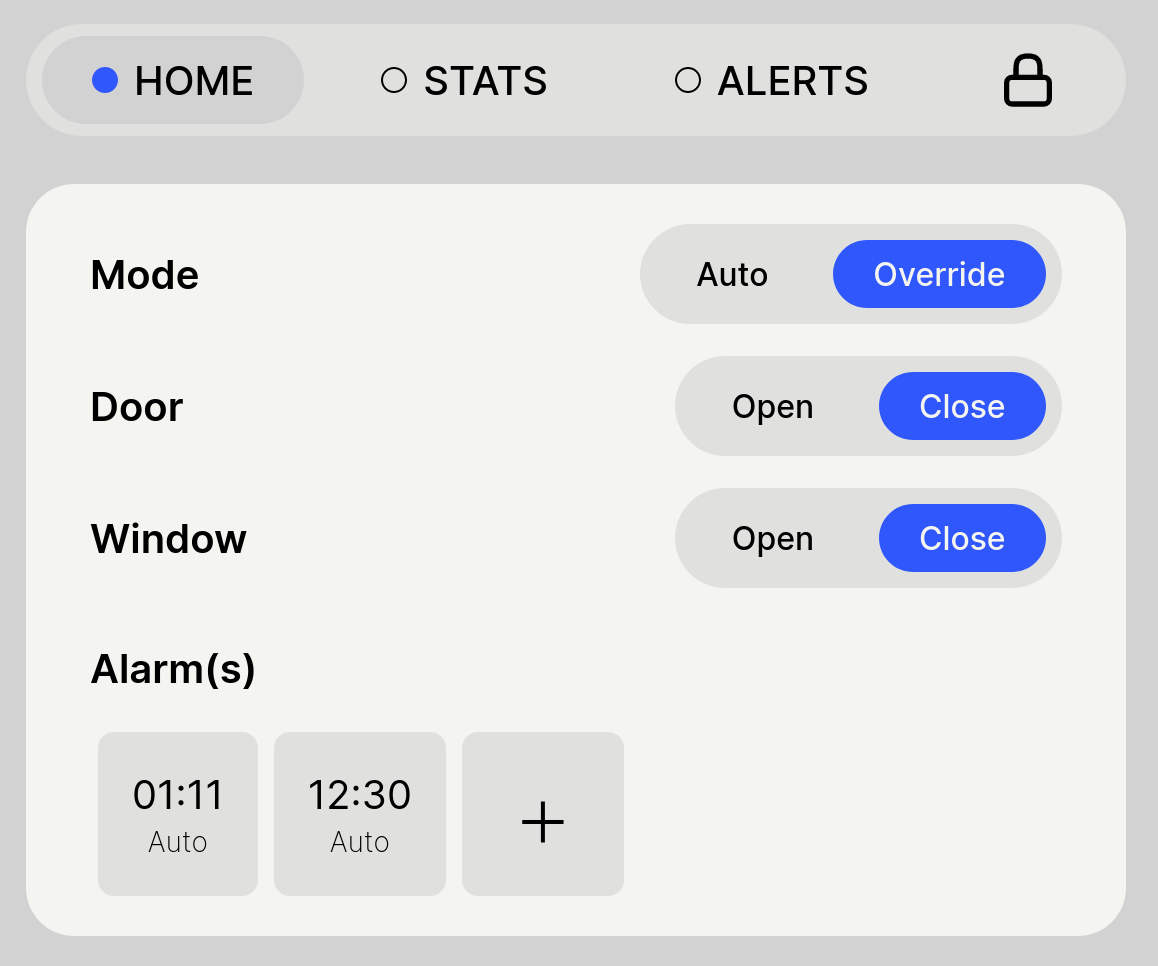
\includegraphics[scale=0.2]{resources/webapp-home-view.png}}
      \caption{Home view of the web application of the smart room air conditioner}
      \label{webapp-home-view}
\end{figure}

\begin{figure}
      \centerline{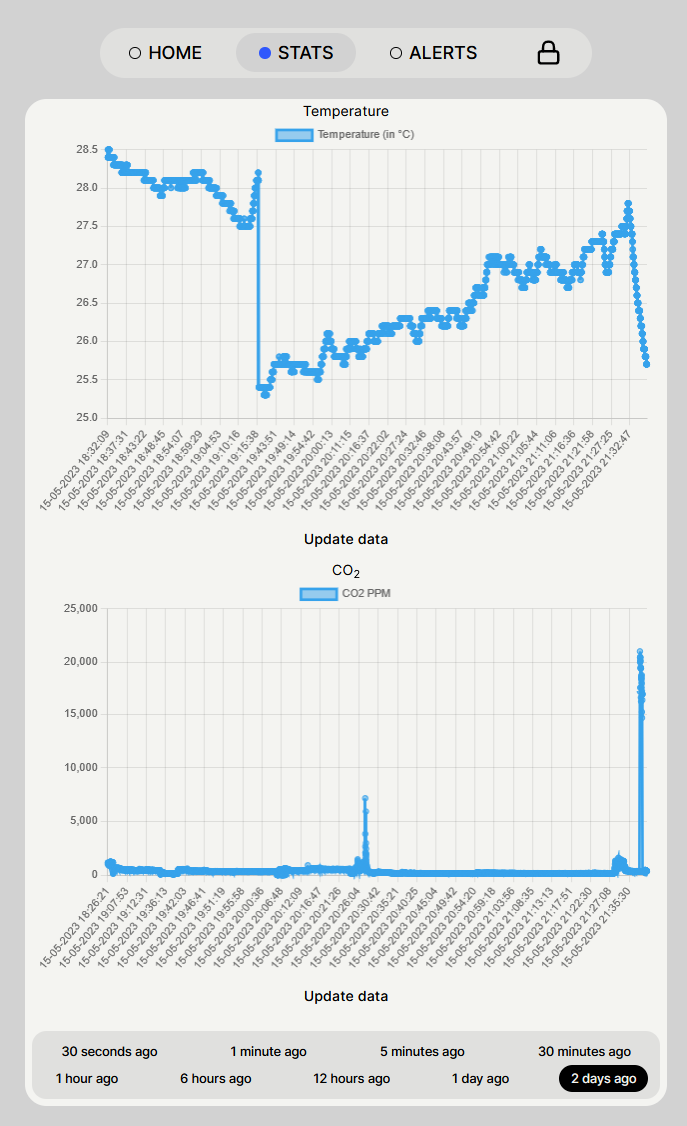
\includegraphics[scale=0.4]{resources/webapp-stats-view.png}}
      \caption{Statistics view of the web application of the smart room air conditioner}
      \label{webapp-stats-view}
\end{figure}

\begin{figure}
      \centerline{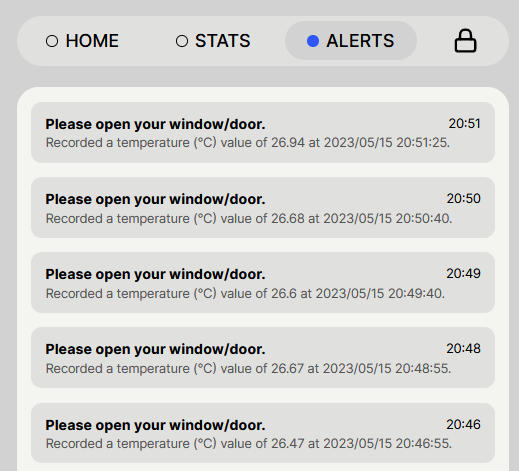
\includegraphics[scale=0.5]{resources/webapp-alerts-view.png}}
      \caption{Alerts view of the web application of the smart room air conditioner}
      \label{webapp-alerts-view}
\end{figure}

\subsection{Discussion}
\subsubsection{Sensors}
The sensors used in the system could detect the
indicators of the air quality, but the accuracy
of the sensors are still questionable.
Specifically, the MQ135 sensor, which is used to
detect the carbon dioxide (CO$_2$) ppm, is not
accurate enough to be used as a reference for.
The MQ135 sensor's base resistance (RZERO) is
not stable, thus affecting the sensor's
reading of the CO$_2$ ppm.

\subsubsection{Machine Learning}
Although the system could already determine to open
or close the door, the system is still far from
perfect. The decision making of opening and closing
the door is merely based on the data from the
sensors and the clustering model. While the actual
air quality of the room related to the health,
comfort, and productivity of the inhabitant are not
considered.

\subsubsection{System Architecture}
Other issues is that, architeturally, the machine
learning model is deployed in the same server with
the application back-end, thus lowering the
performance of the application back-end, when the
machine learning model is being used.

\section{Conclusion and Suggestions}

\subsection{Conclusion}
In this paper, we have presented a system that can be
used to monitor and control the air quality of a room.
The system is able to monitor the air quality of a room,
with temperature and humidity as the indicators; and
the outside, with carbon dioxide (CO$_2$) ppm as the indicator;
and uses those informations to make decision about when to
open and close doors/windows.
The system is also able to be controlled manually via a web
application, and sends notifications to the user's phone
about the state of the system.

\subsection{Suggestions}
The system we proposed is still far from perfect.
There are still many things that can be improved, such as:
\begin{enumerate}
      \item More sophisticated and accurate sensors are
            used.
      \item Health, comfort, and productivity related
            aspects of air quality are considered,
            and not merely depend on the data and
            clustering algorithm.
      \item The machine learning model is deployed
            in a separate server, so that the
            application back-end is not affected
            by the machine learning model.
\end{enumerate}

\section{Conclusion and Suggestions}

\subsection{Conclusion}
In this paper, we have presented a system that can be
used to monitor and control the air quality of a room.
The system is able to monitor the air quality of a room,
with temperature and humidity as the indicators; and
the outside, with carbon dioxide (CO$_2$) ppm as the indicator;
and uses those informations to make decision about when to
open and close doors/windows.
The system is also able to be controlled manually via a web
application, and sends notifications to the user's phone
about the state of the system.

\subsection{Suggestions}
The system we proposed is still far from perfect.
There are still many things that can be improved, such as
\begin{enumerate}
      \item more accurate sensors should be used,
      \item health, comfort, and productivity should be used as parameters in
            the machine learning algorithm, and
      \item the machine learning model should be deployed in a separate service,
            so that the application back-end is decoupled by the prediction
            service by the machine learning model and to improve back-end service
            build time.
\end{enumerate}

\section*{Division of Tasks}

The division of tasks between the member of the group can be
seen in the table \ref{tab-divsion-of-task}.
% Kalau mau dihapus silakan hehe
The tasks are divided based on the member's ability and
willingness to take the issues/features that was listed on GitHub.

\begin{table}[htbp]
	\caption{Division of Tasks}
	\begin{center}
		\begin{tabular}{|c|c|p{3cm}|}
			\hline
			\textbf{Name}    & \textbf{Student ID} & \textbf{Task list}                                                                        \\
			\hline
			Josep Marcello   & 13519164            & \begin{enumerate}[leftmargin=*]
				                                         \item Define system architecture
				                                         \item Calibrate sensors
				                                         \item Setup application and ESP32 boilerplate code
				                                         \item Setup infrastructure (including MQTT, InfluxDB, Telegraf, and Redis)
				                                         \item Connect ESP32 with time server
				                                         \item Develop ESP32 so it's able to control actuator and send sensor data at the same time
				                                         \item Establish connection between ESP32 and application through MQTT
				                                         \item Develop servo toggle feature (back-end)
				                                         \item Develop state manager for application back-end
				                                         \item Develop e-email notification and API to get all sent notifications
				                                         \item Develop simple app password system
				                                         \item Develop (almost realtime) statistics feature
				                                         \item Develop realtime data feature
				                                         \item Integrate ML model to web app
				                                         \item Setup docker for infrastructure and application
				                                         \item Code review
				                                         \item Server donation
			                                         \end{enumerate}
			\\
			\hline
			Jeremia Bachtera & 13519188            & \begin{enumerate}[leftmargin=*]
				                                         \item Define early data pipeline architecture
				                                         \item Develop MQTT-PySpark for data aggregation
				                                         \item Develop mode toggle feature
				                                         \item Develop servo toggle feature (front-end)
				                                         \item Develop websocket to publish current state to front-end clients
				                                         \item Develop, train, and integrate ML model
				                                         \item ``Insert'' ML model to application's back-end
				                                         \item Initiate paper template (with sliced components)
				                                         \item Setup docker for data-pipeline and initial docker-compose
				                                         \item Create Google Slides for progress report
				                                         \item Code review
			                                         \end{enumerate}
			\\
			\hline
			Jeane Erwansyah  & 13519116            & \begin{enumerate}[leftmargin=*]
				                                         \item Determine ML algorithm to use
				                                         \item Design wireframe for web app's UI/UX
				                                         \item Enhance UI/UX of the web app
				                                         \item Develop alerts page
			                                         \end{enumerate}
			\\
			\hline
		\end{tabular}
		\label{tab-divsion-of-task}
	\end{center}
\end{table}
\section*{References}

Please number citations consecutively within brackets \cite{b1}. The
sentence punctuation follows the bracket \cite{b2}. Refer simply to the reference
number, as in \cite{b3}---do not use ``Ref. \cite{b3}'' or ``reference \cite{b3}'' except at
the beginning of a sentence: ``Reference \cite{b3} was the first $\ldots$''

Number footnotes separately in superscripts. Place the actual footnote at
the bottom of the column in which it was cited. Do not put footnotes in the
abstract or reference list. Use letters for table footnotes.

Unless there are six authors or more give all authors' names; do not use
``et al.''. Papers that have not been published, even if they have been
submitted for publication, should be cited as ``unpublished'' \cite{b4}. Papers
that have been accepted for publication should be cited as ``in press'' \cite{b5}.
Capitalize only the first word in a paper title, except for proper nouns and
element symbols.

For papers published in translation journals, please give the English
citation first, followed by the original foreign-language citation \cite{b6}.


\begin{thebibliography}{00}
    \bibitem{productivity_air_quality_wargocki_2000} Wargocki, Pawel \& Wyon, David \& Fanger, P. (2000). Productivity is affected by the air quality in offices. Proceedings of Healthy Buildings 2000. 1.
    \bibitem{indoor_air_quality_stafford_2015} Stafford, Tess. (2015) Indoor Air Quality and Academic Performance. Journal of Environmental Economics and Management. vol. 70. pp. 34-50. doi: 10.1016/j.jeem.2014.10.004.
    \bibitem{iot} Al-Mutawa, Rihab \& Eassa, Fathy. (2020). A Smart Home System based on Internet of Things.

    % Below this is from the template
    \bibitem{b1} G. Eason, B. Noble, and I. N. Sneddon, ``On certain integrals of Lipschitz-Hankel type involving products of Bessel functions,'' Phil. Trans. Roy. Soc. London, vol. A247, pp. 529--551, April 1955.
    \bibitem{b2} J. Clerk Maxwell, A Treatise on Electricity and Magnetism, 3rd ed., vol. 2. Oxford: Clarendon, 1892, pp.68--73.
    \bibitem{b3} I. S. Jacobs and C. P. Bean, ``Fine particles, thin films and exchange anisotropy,'' in Magnetism, vol. III, G. T. Rado and H. Suhl, Eds. New York: Academic, 1963, pp. 271--350.
    \bibitem{b4} K. Elissa, ``Title of paper if known,'' unpublished.
    \bibitem{b5} R. Nicole, ``Title of paper with only first word capitalized,'' J. Name Stand. Abbrev., in press.
    \bibitem{b6} Y. Yorozu, M. Hirano, K. Oka, and Y. Tagawa, ``Electron spectroscopy studies on magneto-optical media and plastic substrate interface,'' IEEE Transl. J. Magn. Japan, vol. 2, pp. 740--741, August 1987 [Digests 9th Annual Conf. Magnetics Japan, p. 301, 1982].
    \bibitem{b7} M. Young, The Technical Writer's Handbook. Mill Valley, CA: University Science, 1989.
\end{thebibliography}


\end{document}
